% ICRA submission -- IEEE conference format.
%
% Build:  latexmk -pdf main.tex        (or: pdflatex main && pdflatex main)
% Figures live in figs/ and are staged from ../figsrc/out and ../pic by
% ../build_icra.py -- do not edit them here.
%
% ANONYMITY: ICRA review policy decides whether the author block below is filled
% in or replaced by "Anonymous submission". Set \anonymoustrue to blind it.
% See ../icra-requirements.md for the confirmed policy for the target edition.

% ICRA 2027 requires the PaperCept `ieeeconf` class, NOT IEEEtran.
% Source: RAS/PaperCept LaTeX support page. See ../icra-requirements.md.
\documentclass[letterpaper, 10 pt, conference]{ieeeconf}

\usepackage[T1]{fontenc}   % ogonek in "St\k{e}pie\'{n}" is unavailable in OT1
\usepackage{cite}
\usepackage{amsmath,amssymb,amsfonts}
\usepackage{graphicx}
\usepackage{booktabs}
\usepackage{url}
\usepackage[table]{xcolor}
\usepackage{microtype}   % subtle tracking/protrusion; buys lines without visible change
\usepackage{balance}

% Default float policy pushes wide floats onto pages of their own, which on this
% paper cost whole pages of white space. Let TeX fill harder before it gives up.
\renewcommand{\topfraction}{0.9}
\renewcommand{\bottomfraction}{0.7}
\renewcommand{\textfraction}{0.1}
\renewcommand{\floatpagefraction}{0.8}
\setcounter{topnumber}{3}
\setcounter{bottomnumber}{2}
\setcounter{totalnumber}{4}

% Tighten the air around floats. IEEE defaults leave a lot of it.
\setlength{\textfloatsep}{5pt plus 1pt minus 1pt}
\setlength{\floatsep}{4pt plus 1pt minus 1pt}
\setlength{\intextsep}{5pt plus 1pt minus 1pt}
\setlength{\abovecaptionskip}{3pt plus 1pt minus 1pt}
\setlength{\belowcaptionskip}{2pt plus 1pt minus 1pt}

\pagestyle{empty}
\thispagestyle{empty}

% Length switches. ICRA 2027 allows 8 pages INCLUDING references; with
% every display item shown this paper runs to 11. Each item below drops
% independently and its switch says what is lost. Rebuild to see the count.
%
% off by default: the raw plots whose numbers a table already carries.
\newif\ifshowJointTable  \showJointTablefalse
\newif\ifshowLoadSweep  \showLoadSweepfalse
\newif\ifshowNyquistTable  \showNyquistTablefalse
\newif\ifshowClosedLoopScatter  \showClosedLoopScatterfalse
\newif\ifshowVelocityTable  \showVelocityTablefalse
\newif\ifshowSpectra  \showSpectrafalse
\newif\ifshowOpenLoopSweep  \showOpenLoopSweepfalse
\newif\ifshowSecondPolicyScatter  \showSecondPolicyScatterfalse

\newif\ifanonymous
% ICRA 2027 review is DOUBLE-ANONYMOUS. Keep this true until acceptance.
\anonymoustrue

\newcommand{\Nm}{\,\mathrm{N}\!\cdot\!\mathrm{m}}
\newcommand{\pending}{\textcolor{orange}{\textsc{[pending]}}}

\begin{document}

\title{\LARGE \bf Decomposing Actuator Thermal Dissipation in Learned Legged
Locomotion: Posture, Ripple, and Closed-Loop Filtering Limits}

% Names, affiliations, identifying links and acknowledgements must be absent from
% the submitted PDF; ICRA 2027 states violations can be desk rejected.
\ifanonymous
  \author{Anonymous submission --- paper ID \pending}
\else
  \author{\pending \thanks{\pending}}
\fi

\maketitle
\thispagestyle{empty}

\begin{abstract}
Reinforcement learning (RL) locomotion policies frequently drive quadrupedal and
humanoid actuators into thermal shutdown by continuously emitting high-rate
position setpoints with high-frequency chattering that exceeds motor bandwidth.
Mitigating this dissipation traditionally requires tedious reward re-tuning and
policy retraining, while post-hoc command smoothing is commonly dismissed due to
filter-induced phase lag that degrades feedback stability margins. In this paper,
we demonstrate that command-side thermal dissipation can be effectively resolved
post-hoc on frozen checkpoints without retraining. We show that electrical copper
loss decomposes in quadrature into a steady-state posture term and a dynamic
ripple term, revealing that their relative dominance is strictly dictated by
joint-specific loading rather than by policy behavior. We identify this crossover
analytically and empirically at $3.2\Nm$ on a Unitree Go1: load-bearing knee
joints sit above this threshold and carry only 14--17\% of their heat in
filter-reachable bands, whereas lightly loaded hip joints sit below it and carry
33--45\%. A Parseval decomposition demonstrates that zero-order-hold staircase
harmonics contribute merely 1.6\% of total heat, with discretionary losses
concentrated in the 5--25\,Hz in-band jitter. While open-loop replay suggests a
46\% thermal reduction via zero-phase filtering, this benefit collapses in closed
loop: a 40\,ms smoothing latency induces falls in 20\% of episodes at 1.0\,m/s on
a regularized policy and in 100\% on an unregularized one. To bypass this latency
penalty, we introduce a causal order-8 predictive filter combined with joint-load
gating. This plug-and-play architecture recovers 47\% and 54\% of the reachable
thermal budget across regularized and unregularized policies without causing
falls. Finally, we show that conventional \texttt{action\_rate} penalties fail to
govern command-side heating (8\% transient increase when ablated), whereas direct
effort and energy penalties dictate the accessible thermal budget (89\% increase).
\end{abstract}

% ieeeconf defines no keywords environment and ICRA does not require one.

\section{Introduction}

Legged locomotion policies trained via deep reinforcement learning (RL)~\cite{lee,miki} routinely
push actuator thermal limits in deployment, frequently triggering thermal
shutdowns in operating regimes where vendor-supplied classical controllers operate
stably. On a Unitree G1 humanoid running whole-body RL, ankle-roll actuators reach
$90\,^\circ$C within minutes of static standing, while the manufacturer's
controller maintains the identical joints below $45\,^\circ$C~\cite{g1issue}.
Conversely, on a wheeled-quadruped Go2-W, a learned policy remains thermally safe
at $60\,^\circ$C while the vendor controller overheats to
$84\,^\circ$C~\cite{go2w}. While it is undeniable that policy behavior governs
motor thermal dissipation, the underlying physical mechanisms driving this
dissipation remain a matter of contention.

Two competing hypotheses are actively debated. Under the \emph{posture
hypothesis}, excessive dissipation stems from high steady-state holding torques
demanded by kinematically inefficient poses. Under the \emph{jitter hypothesis},
dissipation is driven by high-frequency command oscillation---a ubiquitous symptom
in RL policies, which continuously emit discrete-time setpoints that excite
current ripple without producing useful mechanical work.

Neither hypothesis has been rigorously examined because the two mechanisms have
never been evaluated independently. In electric actuators, winding copper loss
scales quadratically with motor torque. Partitioning torque into its mean and
zero-mean fluctuations reveals that posture torque and dynamic ripple add strictly
in quadrature, $\mathcal{H} \propto \mathbb{E}[\tau^2] = \bar{\tau}^2 +
\mathrm{Var}(\tau)$.
Because these terms add in quadrature, a substantial steady-state holding torque
$\bar{\tau}$ mathematically suppresses the relative dissipation contribution of
command variance $\mathrm{Var}(\tau)$. Consequently, whether command jitter
governs heating is not an intrinsic property of the policy, but a state dictated
by joint-specific loading. Both camps are, in fact, observing different joints
across the kinematic chain.

This insight highlights a fundamental engineering dilemma. In standard practice,
researchers attempt to suppress command jitter by laboriously retuning reward
formulations and retraining policies from scratch---a computationally burdensome
and often fragile process, and one that is unavailable whenever the deployed
checkpoint is fixed, as on resource-constrained platforms~\cite{resourceconstrained}. Conversely, deploying post-hoc command smoothing on
frozen checkpoints is traditionally avoided: naive low-pass filtering inevitably
injects phase lag into the feedback path. Because the learned policy operates as a
high-gain feedback controller, this added latency directly erodes closed-loop
stability margins, causing catastrophic falls at operating speeds.

In this paper, we resolve this conflict and demonstrate that command-side thermal
dissipation can be effectively mitigated post-hoc on frozen checkpoints without
retraining. We identify the analytical crossover where steady load overtakes
command ripple, quantify the closed-loop latency boundaries that cause filtered
policies to destabilize, and propose a lightweight, predictive, load-gated filter
that safely recovers the reachable thermal budget.

\subsection{Contributions}

\begin{itemize}
\item \textbf{Spectral heat decomposition.} An exact Parseval-based decomposition
separating actuator dissipation into static posture, gait fundamentals
(0--5\,Hz), in-band jitter (5--25\,Hz), and zero-order-hold (ZOH) discretization
harmonics ($>25$\,Hz). We show that ZOH harmonics account for merely 1.6\% of
heat, identifying the 5--25\,Hz band as the true locus of discretionary
dissipation.
\item \textbf{Quadrature thermal crossover.} We formulate and empirically confirm
the thermal crossover at $\bar{\tau} \approx \sqrt{\mathrm{Var}(\tau)} \approx
3.2\Nm$ on a Unitree Go1, establishing which joints are physically amenable to
filtering.
\item \textbf{Latency failure boundary in closed loop.} Open-loop filtering gains
of up to 46\% evaporate in closed-loop execution. Introducing 40\,ms of filter
latency precipitates a 20\% fall rate at 1.0\,m/s on a regularized policy and
100\% on an unregularized baseline.
\item \textbf{Retraining-free predictive gated filtering.} An order-8 linear
predictive compensator coupled with joint-load gating recovers 47\% and 54\% of
the reachable thermal budget across regularized and unregularized checkpoints
without inducing falls.
\item \textbf{Reward regularization diagnosis.} The conventional
\texttt{action\_rate} penalty has negligible authority over command-side thermal
load (8\% transient increase when ablated), whereas direct torque and energy
penalties dictate the accessible budget (89\% increase).
\end{itemize}

\section{Actuation Pipeline and Problem Formulation}

Commercial quadruped and humanoid architectures execute proportional-derivative
(PD) tracking loops on distributed motor drives rather than within the policy
loop. These drives are quasi-direct-drive: low gear ratios preserve
backdrivability and torque transparency, but leave winding loss directly exposed
to commanded torque~\cite{wensing,minicheetah}, whereas series-elastic designs
place compliance between motor and joint instead~\cite{anymal}. Because neither
is an ideal torque source, sim-to-real pipelines commonly learn the actuator
model from bench data rather than idealizing the joint~\cite{hwangbo}. As illustrated in Fig.~\ref{fig:arch}, the policy emits joint position
targets $q^*$ at frequency $f_{\mathrm{pol}}$. These setpoints cross a
communication bus to motor-side PD loops running at a substantially higher
frequency. In Unitree systems, the policy executes at $f_{\mathrm{pol}} = 50$\,Hz
while low-level commands are written at 500\,Hz~\cite{unitreesdk}; DeepRobotics
Lite3 platforms deploy policies near 83\,Hz over a 1\,kHz state
loop~\cite{lite3blog}. Actuator-level commutation loops run even faster, reaching
6\,kHz on the Unitree GO-M8010-6~\cite{gom8010} and 1\,kHz on the DeepRobotics
J60~\cite{j60}.

\begin{figure*}[!tb]
\centering
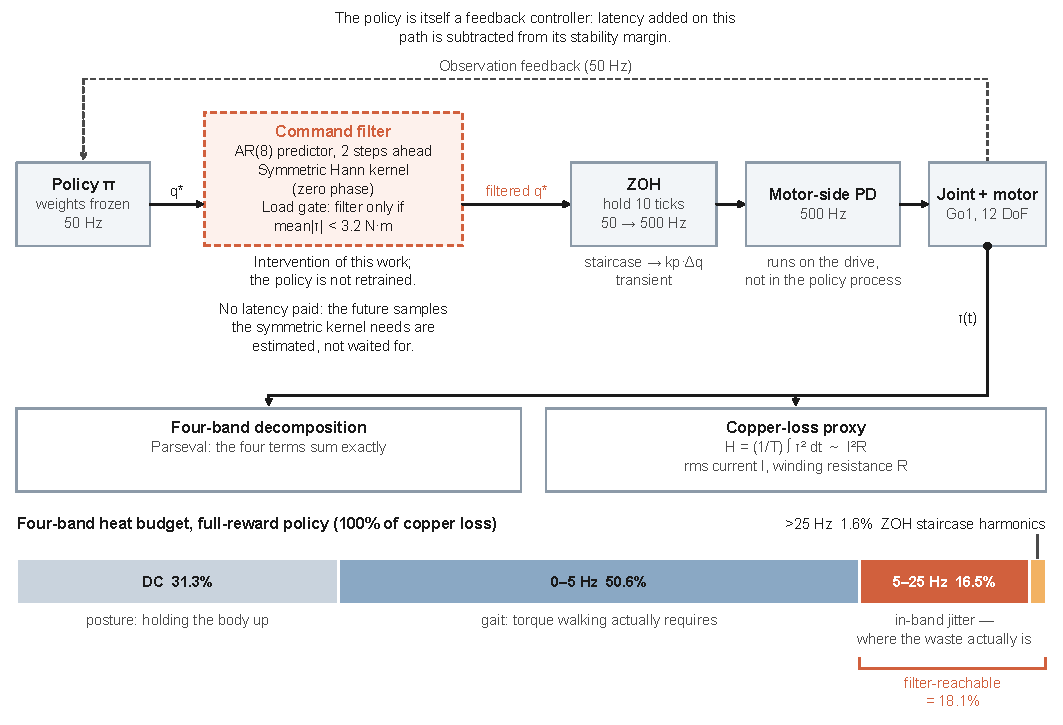
\includegraphics[width=0.82\textwidth]{figs/fig1-architecture.pdf}
\caption{Where the command goes, and where the intervention sits. The policy is
frozen; the only addition is the dashed block. Two details carry the paper: the
torque tap feeding the four-band decomposition, and the dashed feedback path. The
policy is itself a feedback controller, so latency spent inside that loop is
subtracted from its stability margin.}
\label{fig:arch}
\end{figure*}

A zero-order hold (ZOH) sits at the interface between the high-level policy and
low-level drive. Operating at 50\,Hz into 500\,Hz, each setpoint is held constant
across ten sub-ticks before stepping discontinuously, producing an instantaneous
proportional transient of $k_p \Delta q$ prior to mechanical rotor acceleration.

In standardized training environments such as \texttt{unitree\_rl\_mjlab}~\cite{mjlab},
which inherit the manager-based gain and action-scale conventions of Isaac
Lab~\cite{orbit}, PD gains are tuned for a target closed-loop natural frequency of $f_n = 10$\,Hz with
a damping ratio $\zeta = 2.0$, and action scaling is normalized to $0.25\,e/k_p$,
where $e$ is the actuator effort limit. Consequently, an action reversal between
successive policy steps commands a peak transient $\tau_{\mathrm{step}} =
2 k_p (0.25\,e/k_p) = 0.5\,e$.
A full-scale command reversal thus demands an instantaneous torque transient
equivalent to half of the joint's peak effort capacity. With $\zeta = 2.0$, the
dominant closed-loop pole sits at 2.68\,Hz, yet the 50\,Hz command stream
transmits spectral content up to its 25\,Hz Nyquist boundary. The energetic
consequences of this frequency mismatch constitute the core focus of this study.

\section{Metrics and Analytical Framework}

\subsection{Spectral Heat Decomposition}

Applying Parseval's theorem to joint torque partitioned into steady-state and
fluctuating components, total expected dissipation is
\begin{equation}
\begin{split}
\mathbb{E}[\tau^2] = \bar{\tau}^2 &+ \int_{0}^{f_g} S_\tau(f)\,\mathrm{d}f
+ \int_{f_g}^{f_{\mathrm{Nyq}}} S_\tau(f)\,\mathrm{d}f \\
&+ \mathbb{E}_k\!\left[\mathrm{Var}_{\mathrm{sub}}(\tau)\right],
\end{split}
\label{eq:parseval}
\end{equation}
where $f_g = 5$\,Hz isolates fundamental gait frequencies,
$f_{\mathrm{Nyq}} = 25$\,Hz is the policy Nyquist frequency, and
$\mathbb{E}_k[\mathrm{Var}_{\mathrm{sub}}(\tau)]$ represents the intra-step
variance above Nyquist caused by ZOH discretization. The sum of the final two
terms defines the \emph{reachable thermal budget}: the strict upper bound of
dissipation that any command-stream filter can influence.

\subsection{Ripple Fraction and Out-of-Band Power}

When full power spectral density data is unavailable, joint torque fluctuation is
quantified via the joint-level ripple fraction
\begin{equation}
r = \frac{\mathrm{Var}(\tau)}{\bar{\tau}^2 + \mathrm{Var}(\tau)} .
\label{eq:ripple}
\end{equation}
Independent of plant dynamics, command-side roughness is characterized by the
out-of-band command power fraction
\begin{equation}
\rho = \frac{\int_{f_c}^{f_{\mathrm{Nyq}}} S_q(f)\,\mathrm{d}f}
            {\int_{0}^{f_{\mathrm{Nyq}}} S_q(f)\,\mathrm{d}f} ,
\label{eq:rho}
\end{equation}
where $f_c$ is the joint's $-3$\,dB closed-loop bandwidth, 15.3\,Hz for the
Unitree Go1 model. A coarser metric evaluated at 5\,Hz, denoted
$\rho_{>5\,\mathrm{Hz}}$, is also used to track broadband high-frequency content.
The two are different cuts and are not interchangeable.

\subsection{Thermal Loss Proxy}

Motor thermal dissipation is quantified via
$\mathcal{H} = \frac{1}{T}\int_0^T \tau^2\,\mathrm{d}t$, proportional to winding
copper loss $I_{\mathrm{rms}}^2 R$ under a constant torque sensitivity $K_t$.
Quadratic torque evaluation is physically validated by stator thermal dynamics: on
calibrated brushless actuators, the winding thermal time constant is 3.12\,s
against 777\,s for the motor housing---a disparity factor of 249~\cite{maxon}.
Because driver thermistors exhibit significant thermal lag relative to winding
junctions, and because driver-reported temperature is itself the output of a
model rather than a winding measurement~\cite{wallscheid,kirchgassner,thermalpred},
current-based squared torque serves as the primary ground-truth
metric~\cite{urs}. Minimizing $I^2R$ is likewise the drive-side statement of
energy-efficient motor control~\cite{energymotor}.

\subsection{Effect Size}

Paired comparisons between schemes are reported with Cliff's $\delta$, a
non-parametric ordinal effect size that makes no distributional
assumption~\cite{cliff}.

\section{Experimental Setup}

Four experimental protocols are evaluated. The labels follow the source
experiments; there is no E4, as the label was never assigned. The checkpoints and
the reward-term vocabulary the ablations manipulate follow the massively parallel
GPU training practice of \texttt{legged\_gym}~\cite{rudin} on Isaac
Gym~\cite{isaacgym} and the open sim-to-real stacks published for the
Go1~\cite{wtw}.

\textbf{E1 (single joint, synthetic signals).} A second-order joint model
representative of the Unitree Go1~\cite{playground} ($k_p = 35$, damping 0.5, rotor inertia
0.005\,kg$\cdot$m$^2$, $f_n = 13.3$\,Hz, $\zeta = 0.60$, $-3$\,dB bandwidth
15.3\,Hz) is excited by a 2\,Hz sinusoidal command injected with bandpass noise
above bandwidth. Commands are sampled at 50\,Hz, held via ZOH to 500\,Hz, and
integrated at 5\,kHz. Static load torques are swept from 0 to $20\Nm$.

\textbf{E2 (recorded trajectories, open loop).} Trajectories logged from seven Go1
policies across reward ablations are replayed through the single-joint model under
candidate filter configurations. Preserved motion is benchmarked against the ZOH
trajectory low-passed at 5\,Hz.

\textbf{E3 (closed loop, full quadruped).} A frozen Go1 policy is executed in
MuJoCo at a 50\,Hz policy rate and 500\,Hz physics rate, ten substeps per policy
step, with the candidate filtering pipeline active inside the feedback loop. Ten
500-step episodes are evaluated at each of three velocity commands (0.5\,m/s,
1.0\,m/s, and 0.3\,m/s with yaw rate) across matched seeds and observation noise,
giving $n = 30$ per scheme.

\textbf{E5 (spectral decomposition).} Identical to E3 under baseline ZOH over 30
rollouts. Mean torque per policy step is recorded at 50\,Hz, with spectral cuts at
5\,Hz and 25\,Hz, and intra-step variance supplying the $>25$\,Hz component.

\textbf{Predictive compensator and load gate.} An order-8 linear autoregressive
model, AR(8), is fitted by least squares on baseline rollouts in the standard
linear-prediction sense~\cite{makhoul} and rolled forward
two steps. This enables a symmetric Hann window~\cite{harris} to be applied without awaiting
future samples, eliminating filter phase lag (Fig.~\ref{fig:filters}). Joints
whose mean absolute torque $|\bar{\tau}|$ falls below the $3.2\Nm$ threshold are
filtered, whereas heavily loaded joints pass through unmodified.

\begin{figure}[!tb]
\centering
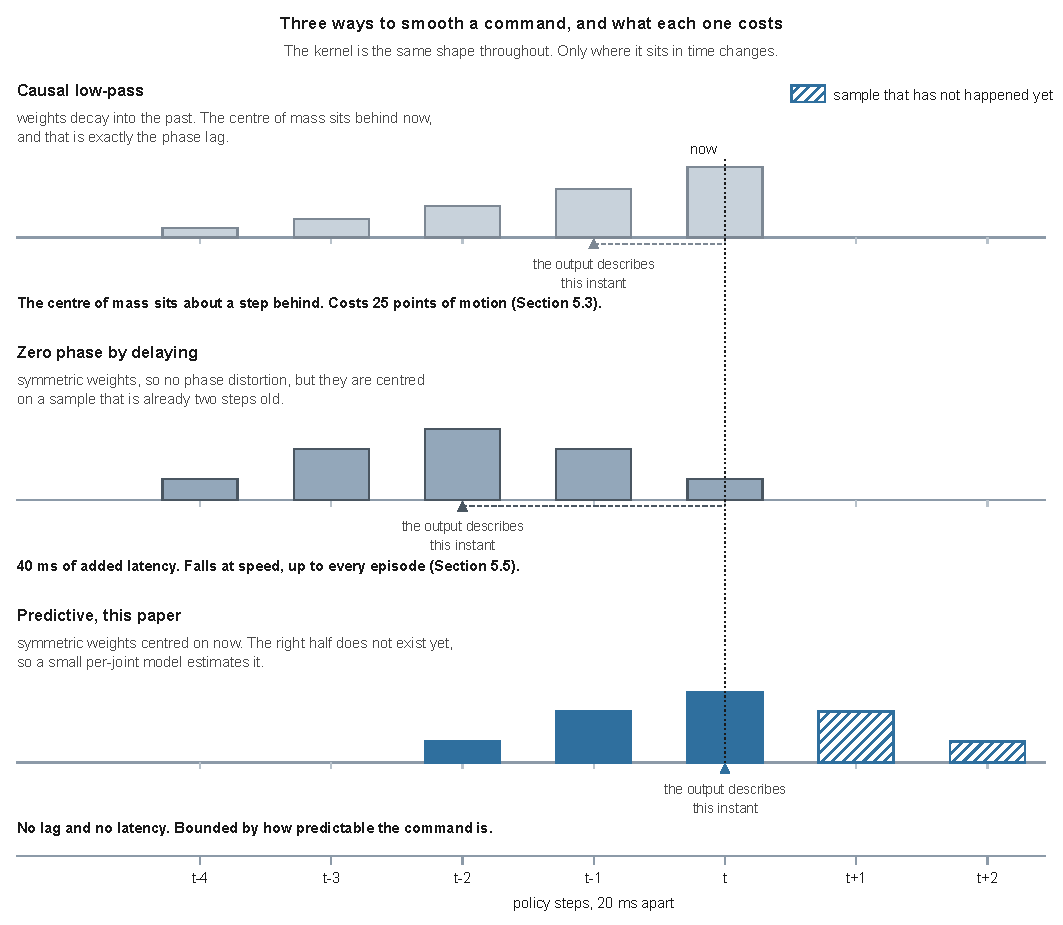
\includegraphics[width=0.95\columnwidth]{figs/fig5-three-filters.pdf}
\caption{Three ways to smooth a command, and what each one costs. The kernel is
the same shape throughout; only where it sits in time changes. The causal filter's
centre of mass sits behind now, and that gap \emph{is} the phase lag. Delaying two
steps recovers symmetry but spends 40\,ms of latency out of the policy's stability
margin. The predictive filter keeps the kernel centred on now and estimates the
half that has not happened yet.}
\label{fig:filters}
\end{figure}

\section{Results and Empirical Analysis}

\subsection{Load-Dependent Thermal Crossover}

Holding kinematic motion amplitude constant, the thermal penalty of out-of-band
command power scales inversely with static load (Table~\ref{tab:e1}).

\begin{table}[!tb]
\caption{Thermal dissipation relative to $\rho = 0$ across static load levels
under single-joint excitation (E1).}
\label{tab:e1}
\centering
\footnotesize
\setlength{\tabcolsep}{3pt}
\begin{tabular}{lrrrrr}
\toprule
Static load & $\rho{=}0.02$ & $0.05$ & $0.10$ & $0.20$ & $0.40$ \\
\midrule
$0\Nm$  & 1.81 & 3.08 & 5.38 & \textbf{10.86} & 27.30 \\
$2\Nm$  & 1.15 & 1.40 & 1.84 & 2.89  & 6.04 \\
$5\Nm$  & 1.03 & 1.08 & 1.16 & 1.36  & 1.96 \\
$10\Nm$ & 1.01 & 1.02 & 1.04 & 1.09  & 1.25 \\
$20\Nm$ & 1.00 & 1.00 & 1.01 & \textbf{1.02}  & 1.06 \\
\bottomrule
\end{tabular}
\end{table}

\ifshowLoadSweep  % off: loses the rho/(1-rho) linearity and its 0.45 percent residual
\begin{figure*}[!tb]
\centering
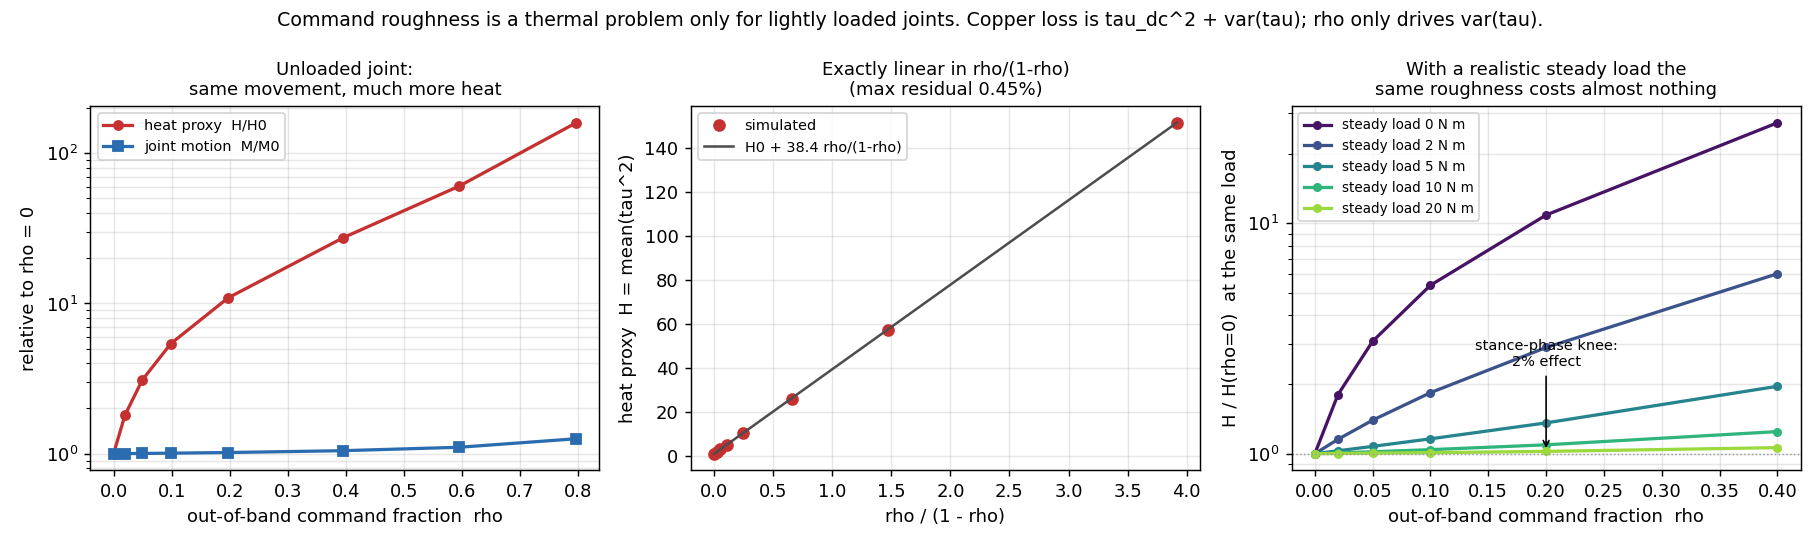
\includegraphics[width=0.82\textwidth]{figs/e1-rho-sweep.png}
\caption{Single-joint load sweep (E1). Left: with no load, heat climbs steeply
with out-of-band command power while the joint's motion does not. Centre: the
relationship is exactly linear in $\rho/(1-\rho)$, maximum residual 0.45\%. Right:
a realistic steady load flattens it almost completely.}
\label{fig:e1}
\end{figure*}
\fi

At $\rho = 0.20$, an unloaded joint dissipates 10.9 times the heat of an
uncorrupted command while altering joint motion by only 1.8\%. In contrast, a
joint supporting a $20\Nm$ static load exhibits merely a 2\% thermal increase under
the same command roughness. Under unloaded conditions, dissipation follows
\begin{equation}
\mathcal{H} = \mathcal{H}_0 + \kappa\,\frac{\rho}{1-\rho}
\label{eq:kappa}
\end{equation}
with $\kappa = 38.4$ and a maximum residual of 0.45\%. The crossover where posture
loss equals ripple loss, $\bar{\tau}^2 = \mathrm{Var}(\tau)$, emerges at $3.2\Nm$.

On the Unitree Go1, measured mean absolute joint torques $|\bar{\tau}|$ average
1.24--1.48$\Nm$ for hip abduction, 2.00--2.59$\Nm$ for thighs, and
5.88--6.88$\Nm$ for calves. Eight of the twelve joints operate below the $3.2\Nm$
crossover, while the four knee actuators operate well above it
(Fig.~\ref{fig:crossover}). Motor selection for quasi-direct-drive joints is
argued on the same footing, by the torque operating point rather than by peak
rating~\cite{motorselect}. Consequently, posture demands dominate knee
dissipation, whereas jitter drives overheating in lightly loaded joints.

\begin{figure}[!tb]
\centering
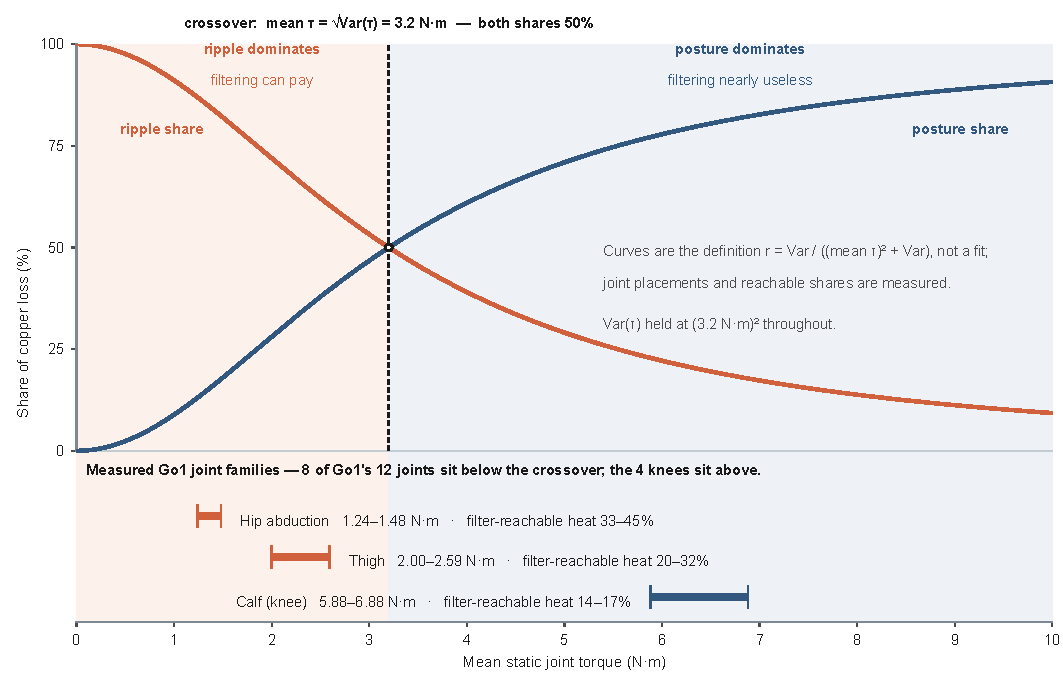
\includegraphics[width=0.95\columnwidth]{figs/fig2-crossover.pdf}
\caption{The quadrature crossover. Which term dominates is a property of the
joint, not of the policy. The curves are the definition
$r = \mathrm{Var}/(\bar{\tau}^2+\mathrm{Var})$, not a fit; the joint placements and
reachable shares are measured.}
\label{fig:crossover}
\end{figure}

\subsection{Effort Terms Govern Jitter; Action Rate Does Not}

Command-side statistics were evaluated across ablated Go1 policy checkpoints
(single-seed, 8\,s rollouts). Table~\ref{tab:ablation} reports five representative
variants of the seven trained; statistics for the remaining two are \pending.

\begin{table}[!tb]
\caption{Command-side spectral properties across reward ablations (E2).
$\rho_{>5\,\mathrm{Hz}}$ is the coarse 5\,Hz cut, not the $-3$\,dB-bandwidth
$\rho$.}
\label{tab:ablation}
\centering
\footnotesize
\setlength{\tabcolsep}{3pt}
\begin{tabular}{lrrrr}
\toprule
Policy variant & $\Delta q_{\mathrm{rms}}$ & $\tau_{\mathrm{step}}$ RMS & Centroid & $\rho_{>5\,\mathrm{Hz}}$ \\
 & (rad) & ($\mathrm{N}\!\cdot\!\mathrm{m}$) & (Hz) & \\
\midrule
Full reward           & 0.0668 & 2.34 & 3.29  & 0.051 \\
No \texttt{act\_rate} & 0.0723 & \textbf{2.53} ({+}8\%) & 3.43 & 0.119 \\
No gait terms         & 0.0747 & 2.62 ({+}12\%) & 4.98 & 0.146 \\
No torque+energy & 0.1267 & \textbf{4.43} ({+}89\%) & 5.44 & 0.363 \\
Task terms only       & 0.1586 & 5.55 ({+}137\%) & 10.44 & 0.898 \\
\bottomrule
\end{tabular}
\end{table}

\ifshowSpectra  % off: loses raw command spectra; Table II carries the numbers
\begin{figure*}[!tb]
\centering
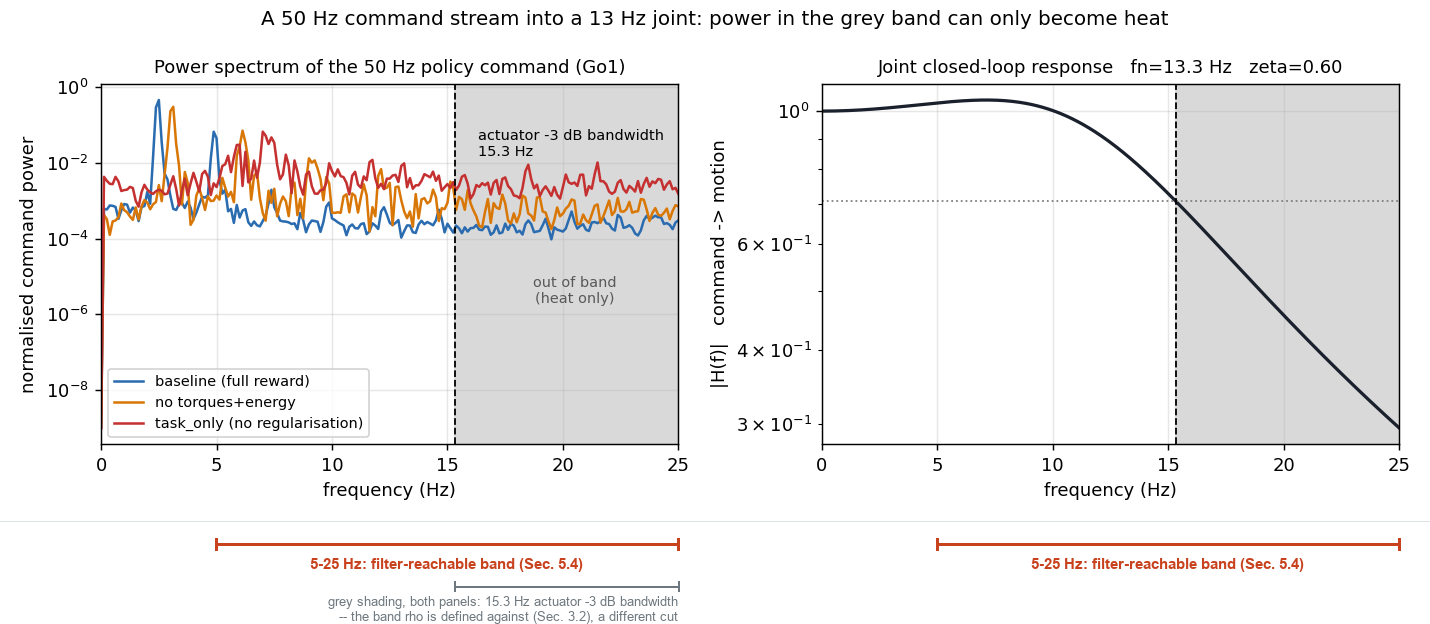
\includegraphics[width=0.82\textwidth]{figs/command-spectrum-annotated.png}
\caption{Command spectra across reward ablations. The unregularized policy is flat
across the whole band. The grey shading is the 15.3\,Hz actuator bandwidth that
$\rho$ is defined against---\emph{not} the 5--25\,Hz filter-reachable band, which
the rule below the axes marks instead.}
\label{fig:spectrum}
\end{figure*}
\fi

Ablating the standard \texttt{action\_rate} penalty increases step transients by
only 8\%. Conversely, eliminating joint torque and energy regularizations inflates
step transients by 89\%. Direct effort minimization, rather than discrete action
smoothing, serves as the primary regularizer of command-side thermal load. The
same lever has been made adaptive to drive gait transition and locomotion
efficiency~\cite{energyreg}.

\subsection{Open-Loop Filtering and the Cost of Phase Lag}

Replaying baseline trajectories through the unloaded single-joint model
demonstrates the apparent efficacy of open-loop smoothing
(Table~\ref{tab:openloop}).

\begin{table}[!tb]
\caption{Open-loop command replay through an unloaded joint model (E2).}
\label{tab:openloop}
\centering
\footnotesize
\setlength{\tabcolsep}{3pt}
\begin{tabular}{lrrc}
\toprule
Scheme & $\mathcal{H}/\mathcal{H}_{\mathrm{ZOH}}$ & Motion & Depl. \\
\midrule
Baseline ZOH                    & 1.000 & 1.000 & --- \\
Linear interpolation            & 0.696 & 0.819 & Yes \\
Causal Butter. (12\,Hz)     & 0.588 & 0.745 & Yes \\
Predictive filter               & \textbf{0.428} & 0.741 & Yes \\
Zero-phase Butter. (12\,Hz) & 0.540 & \textbf{0.995} & No \\
\bottomrule
\end{tabular}
\end{table}

\ifshowOpenLoopSweep  % off: loses raw open-loop sweep; Table III carries the numbers
\begin{figure*}[!tb]
\centering
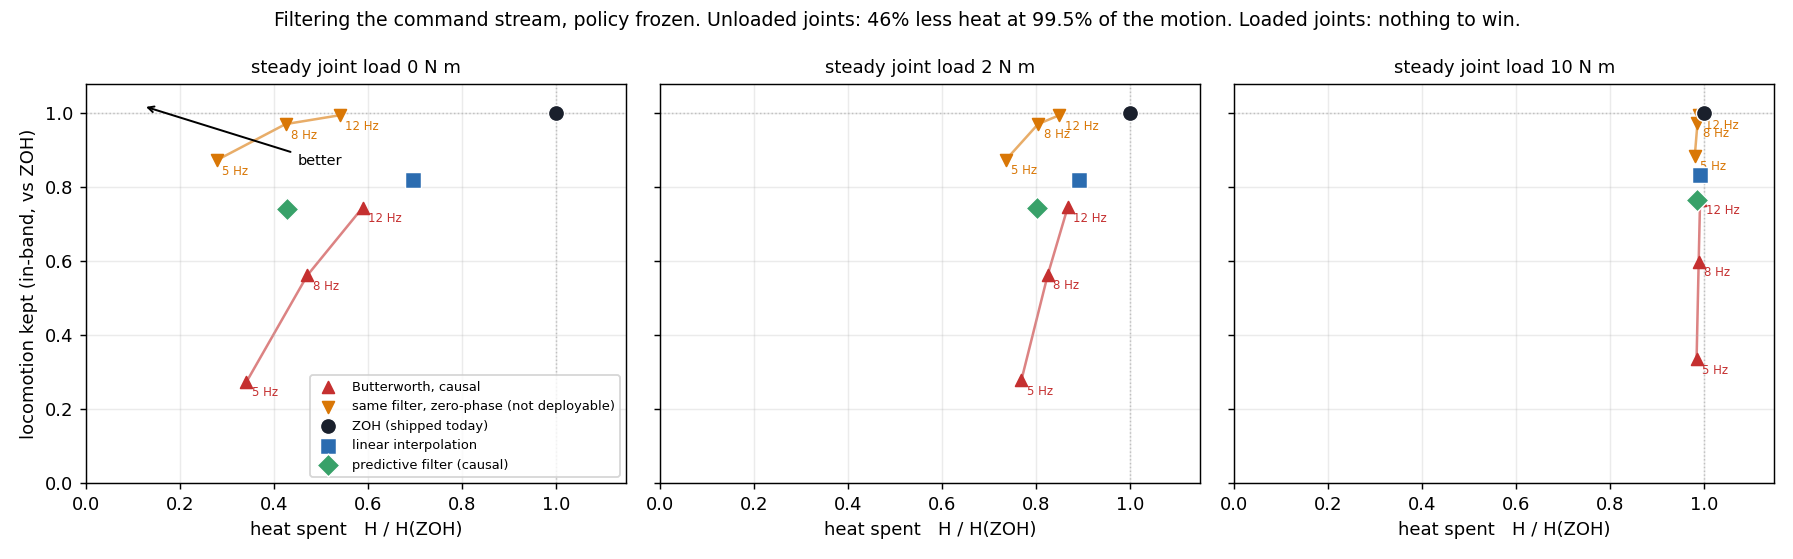
\includegraphics[width=0.82\textwidth]{figs/e3-command-filters.png}
\caption{Open-loop filter sweep (E2). Up and to the left is better. The zero-phase
curve dominates the causal one at every cutoff, and the gap between them is phase
lag alone. At $10\Nm$ of steady load the whole picture collapses to a vertical
line: there is nothing to win.}
\label{fig:openloop}
\end{figure*}
\fi

Zero-phase filtering---non-causal, because the record is run through the filter
forwards and then backwards~\cite{gustafsson}---achieves a 46\% thermal reduction
while preserving 99.5\% of intended trajectory motion. However, a causal implementation of the identical
filter preserves only 74.5\% of intended motion due entirely to phase lag.
Out-of-sample \emph{open-loop} command prediction accuracy reaches $R^2 = 0.679$
on the full-reward policy, declining to 0.385 without effort terms, and collapsing
to 0.059 on an unregularized checkpoint. A separate predictor fitted for the
closed-loop experiments reports different values (Table~\ref{tab:policies}).

\subsection{Spectral Allocation of the Thermal Budget}

Exact Parseval decomposition across 30 closed-loop rollouts sets the theoretical
ceiling for command filtering (Table~\ref{tab:bands}).

\begin{table}[!tb]
\caption{Exact closed-loop torque spectral decomposition across 30 rollouts on the
baseline Go1 policy (E5). The four components sum to 255.9 against an
independently computed heat proxy of 256.2.}
\label{tab:bands}
\centering
\footnotesize
\setlength{\tabcolsep}{3pt}
\begin{tabular}{llr}
\toprule
Band & Physical mechanism & Share \\
\midrule
DC          & Posture: static body support        & 31.3\% \\
0--5\,Hz    & Gait: torque walking requires       & 50.6\% \\
5--25\,Hz   & In-band jitter: filter-reachable    & 16.5\% \\
$>25$\,Hz   & ZOH staircase harmonics             & 1.6\% \\
\midrule
\textbf{Total reachable} & Jitter and harmonics combined & \textbf{18.1\%} \\
\bottomrule
\end{tabular}
\end{table}

The ZOH staircase---the explicit focus of interpolation literature---accounts for
only 1.6\% of motor dissipation. Discretionary thermal waste resides primarily
between 5 and 25\,Hz. As predicted by the crossover, the reachable budget scales
inversely with joint holding load\ifshowJointTable (Table~\ref{tab:joints})\fi: lightly loaded hip
actuators reach 33--45\%, while weight-bearing calf actuators remain confined to
14--17\%.

\ifshowJointTable  % off: loses per-joint-family reachable shares, which the abstract quotes
\begin{table}[!tb]
\caption{Joint-specific torque budget decomposition (E5). Reachable share is the
sum of the 5--25\,Hz and $>25$\,Hz columns.}
\label{tab:joints}
\centering
\footnotesize
\setlength{\tabcolsep}{3pt}
\begin{tabular}{lrrrrrr}
\toprule
Joint & $|\bar{\tau}|$ & DC & Gait & 5--25 & $>25$ & Reach. \\
family & ($\mathrm{N}\!\cdot\!\mathrm{m}$) & & & Hz & Hz & \\
\midrule
Hips    & 1.2--1.5 & 7--21\%  & 47--54\% & 33--45\% & 0.3--0.4\% & \textbf{33--45\%} \\
Thighs  & 2.0--2.6 & 2--19\%  & 56--78\% & 16--29\% & 3.0--4.0\% & \textbf{20--32\%} \\
Calves  & 5.9--6.9 & 32--38\% & 45--54\% & 13--16\% & 1.1--1.6\% & \textbf{14--17\%} \\
\bottomrule
\end{tabular}
\end{table}
\fi

\begin{figure*}[!tb]
\centering
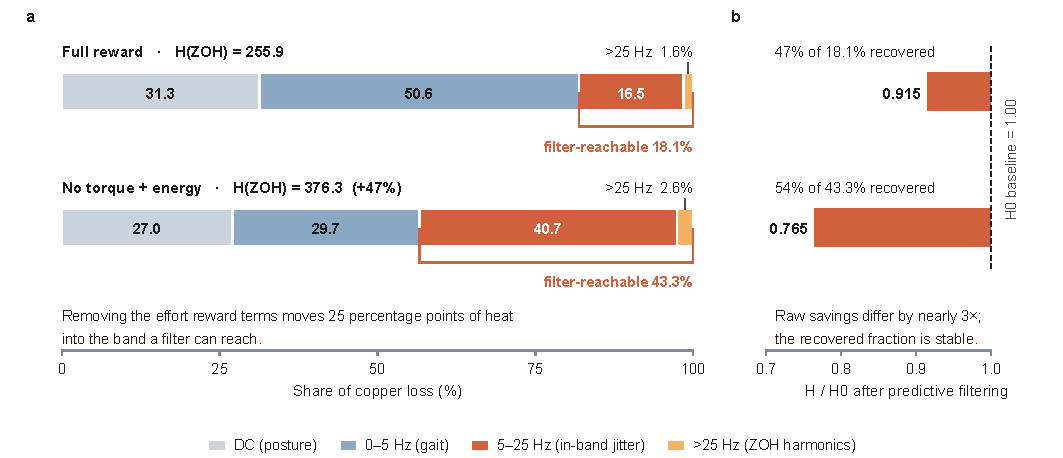
\includegraphics[width=0.82\textwidth]{figs/fig3-band-budget.pdf}
\caption{The heat budget, both policies. The $>25$\,Hz sliver is drawn to scale:
that is what 1.6\% looks like. Removing the effort reward terms moves 25
percentage points of heat into the band a filter can reach, and the filter returns
about half of whatever is there on either policy.}
\label{fig:budget}
\end{figure*}

\subsection{Closed-Loop Filtering: Latency Induces Instability}

When deployed inside the active feedback control loop, open-loop filtering gains
evaporate due to phase lag (Table~\ref{tab:closedloop}). The policy is itself a
feedback controller, trained alongside the state estimator that closes the same
loop~\cite{concurrent}, so latency inserted ahead of it is taken out of its own
phase margin.

\begin{table}[!tb]
\caption{Full-body closed-loop locomotion performance ($n = 30$ per scheme, E3).
Cliff's $\delta$ is reported against ZOH.}
\label{tab:closedloop}
\centering
\footnotesize
\setlength{\tabcolsep}{3pt}
\begin{tabular}{lrrrrr}
\toprule
Scheme & $\mathcal{H}/\mathcal{H}_{\mathrm{ZOH}}$ & Track. & $\delta(H)$ & $\delta(v)$ & Fall \\
\midrule
Baseline ZOH              & 1.000 & 1.000 & 0.00 & 0.00 & 0.00 \\
Linear interpolation      & 0.956 & 1.048 & $-0.31$ & 0.13 & 0.00 \\
Butterworth (5\,Hz) & 1.098 & 2.594 & $-0.04$ & 1.00 & \textbf{0.23} \\
Butterworth (8\,Hz) & 0.946 & 1.444 & $-0.28$ & 0.93 & 0.00 \\
Butterworth (12\,Hz) & 0.935 & 1.160 & $-0.28$ & 0.52 & 0.00 \\
Butter. 12\,Hz + lin. & 0.942 & 1.284 & $-0.26$ & 0.75 & 0.00 \\
Zero-phase, 40\,ms & \textbf{1.082} & 2.493 & $-0.03$ & 1.00 & \textbf{0.07} \\
Predictive filter         & \textbf{0.915} & 1.279 & $-0.33$ & 0.71 & 0.00 \\
Predictive + joint gate   & 0.940 & 1.157 & $-0.33$ & 0.50 & 0.00 \\
Predictive, policy-unaw. & 0.927 & 1.236 & $-0.33$ & 0.64 & 0.00 \\
\bottomrule
\end{tabular}
\end{table}

\ifshowClosedLoopScatter  % off: loses the heat-vs-tracking trade-off and which joints the gate touches
\begin{figure*}[!tb]
\centering
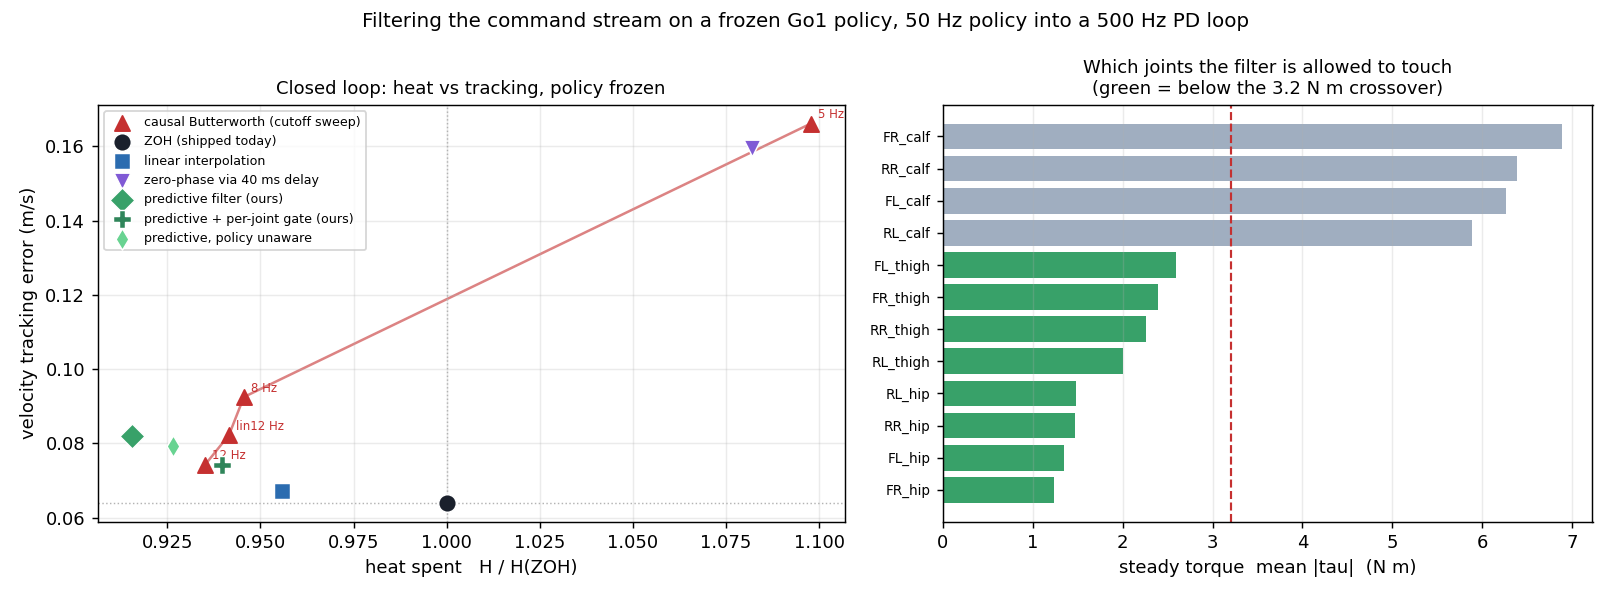
\includegraphics[width=0.82\textwidth]{figs/e4-closed-loop.png}
\caption{Closed loop, full-reward policy (E3). Heat against tracking error with
the filter inside the loop. Right panel: which joints the gate lets the filter
touch. The four calves sit above the $3.2\Nm$ line and pass through untouched.}
\label{fig:closedloop}
\end{figure*}
\fi

The predictive filter achieves an 8.5\% total thermal reduction (Cliff's
$\delta = -0.33$), representing a 47\% recovery of the 18.1\% reachable budget. In
contrast, linear interpolation recovers only 4.4\% of total heat.

Filtering the ZOH staircase harmonics does not drive overall thermal recovery\ifshowNyquistTable (Table~\ref{tab:nyquist})\fi. Schemes that halve the $>25$\,Hz term generate higher
net thermal dissipation, whereas the predictive filter leaves staircase harmonics
untouched and attains the lowest total heat.

\ifshowNyquistTable  % off: loses the evidence that halving the staircase term raises total heat
\begin{table}[!tb]
\caption{Actuator dissipation above Nyquist compared to total thermal load.}
\label{tab:nyquist}
\centering
\footnotesize
\setlength{\tabcolsep}{3pt}
\begin{tabular}{lrr}
\toprule
Scheme & $>25$\,Hz term & Total $\mathcal{H}/\mathcal{H}_0$ \\
\midrule
Baseline ZOH             & 4.02 & 1.000 \\
Butterworth (5\,Hz)      & \textbf{1.96} & \textbf{1.098} \\
Zero-phase, 40\,ms delay & \textbf{2.34} & \textbf{1.082} \\
Butterworth (12\,Hz)     & 2.93 & 0.935 \\
Predictive filter        & 4.02 & \textbf{0.915} \\
\bottomrule
\end{tabular}
\end{table}
\fi

\ifshowVelocityTable  % off: loses exact per-velocity fall rates behind contribution C3
\begin{table}[!tb]
\caption{Velocity-dependent performance and failure rates,
$\mathcal{H}/\mathcal{H}_0$ (fall rate) (E3).}
\label{tab:velocity}
\centering
\footnotesize
\setlength{\tabcolsep}{3pt}
\begin{tabular}{lrrr}
\toprule
Scheme & 0.5\,m/s & 1.0\,m/s & 0.3\,m/s + turn \\
\midrule
Zero-phase, delay & 0.883 (0.00) & \textbf{1.258 (0.20)} & 0.992 (0.00) \\
Butterworth (5\,Hz) & 0.880 (0.00) & \textbf{1.295 (0.70)} & 0.991 (0.00) \\
Predictive + gate & 0.952 (0.00) & 0.924 (0.00) & 0.956 (0.00) \\
Predictive + gate, track. & 1.298 & 0.995 & 1.250 \\
\bottomrule
\end{tabular}
\end{table}
\fi

\begin{figure*}[!tb]
\centering
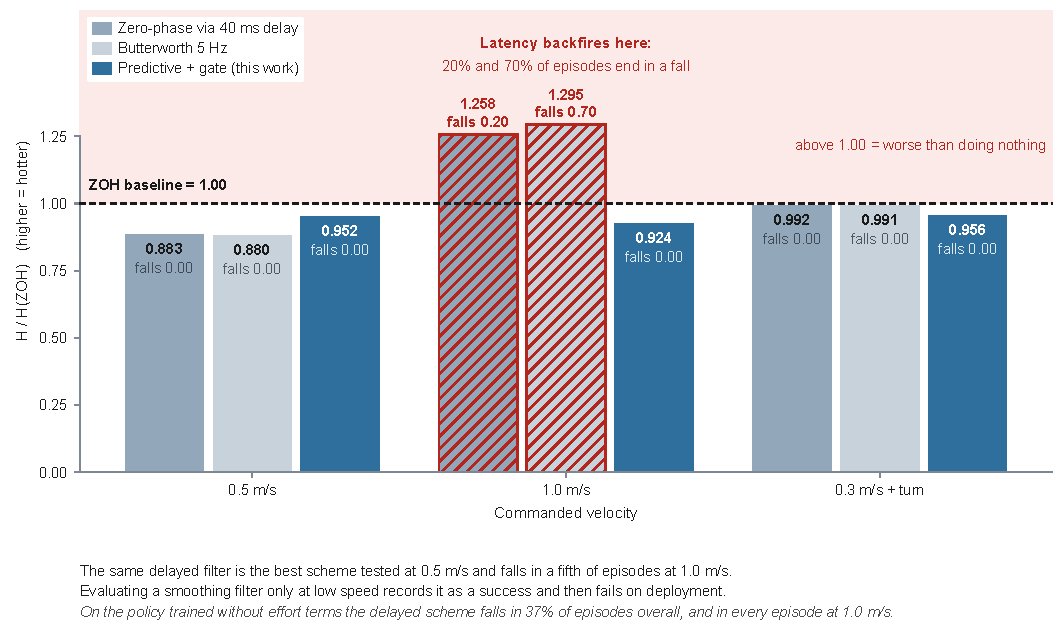
\includegraphics[width=0.82\textwidth]{figs/fig4-latency-backfire.pdf}
\caption{Latency backfires, and only at speed. The same delayed filter is the best
scheme tested at 0.5\,m/s and falls in a fifth of episodes at 1.0\,m/s. Bars above
the ZOH baseline are worse than doing nothing. This argues against evaluating a
smoothing filter at the bottom of the speed range.}
\label{fig:latency}
\end{figure*}

The delayed zero-phase filter succeeds at 0.5\,m/s, with a 12\% heat reduction and
zero falls, but destabilizes at 1.0\,m/s, with a 20\% fall rate and a 25.8\% heat
increase\ifshowVelocityTable (Table~\ref{tab:velocity})\fi. Similarly, the 5\,Hz Butterworth induces
falls in 70\% of episodes at 1.0\,m/s. Delay is not unmanageable in principle---%
model-based agents absorb it by augmenting the state with the pending action
queue~\cite{delayaware}---but that route requires retraining, whereas real-time
chunking hides inference latency by inpainting the next chunk rather than
delaying execution~\cite{rtc}. Gating the predictive filter by joint load
costs 2.5 percentage points of thermal relief but maintains tracking fidelity at
0.995 of baseline at 1.0\,m/s without falls.

\subsection{Invariant Recovery Ratio on Unregularized Policies}

Evaluating the closed-loop pipeline on an unregularized policy, trained without
torque or energy penalties, demonstrates consistent budget recovery
(Table~\ref{tab:policies}).

\begin{table}[!tb]
\caption{Regularized against effort-ablated policies (E3, E5). The predictor
$R^2$ row is the closed-loop fit; the open-loop fit is a different quantity.}
\label{tab:policies}
\centering
\footnotesize
\setlength{\tabcolsep}{3pt}
\begin{tabular}{lrr}
\toprule
Metric & Full reward & No effort \\
\midrule
Baseline ZOH heat & 255.9 & \textbf{376.3} ({+}47\%) \\
Bands DC/gait/5--25/$>$25 & 31.3/50.6/16.5/1.6 & 27.0/29.7/40.7/2.6 \\
Filter-reachable share & \textbf{18.1\%} & \textbf{43.3\%} \\
Command predictor $R^2$ & 0.609 & 0.402 \\
Predictive $\mathcal{H}/\mathcal{H}_0$ & 0.915 & \textbf{0.765} \\
Recovered / reachable & \textbf{47\%} & \textbf{54\%} \\
Pred.\ + gate $\mathcal{H}/\mathcal{H}_0$ & 0.940 & 0.879 \\
Pred.\ + gate tracking & 1.157 & 1.149 \\
Zero-phase $\mathcal{H}/\mathcal{H}_0$ & 1.082 & 1.053 \\
Zero-phase fall rate & 0.07 & \textbf{0.37} \\
\bottomrule
\end{tabular}
\end{table}

\ifshowSecondPolicyScatter  % off: loses second-policy scatter; Table IX carries the numbers
\begin{figure*}[!tb]
\centering
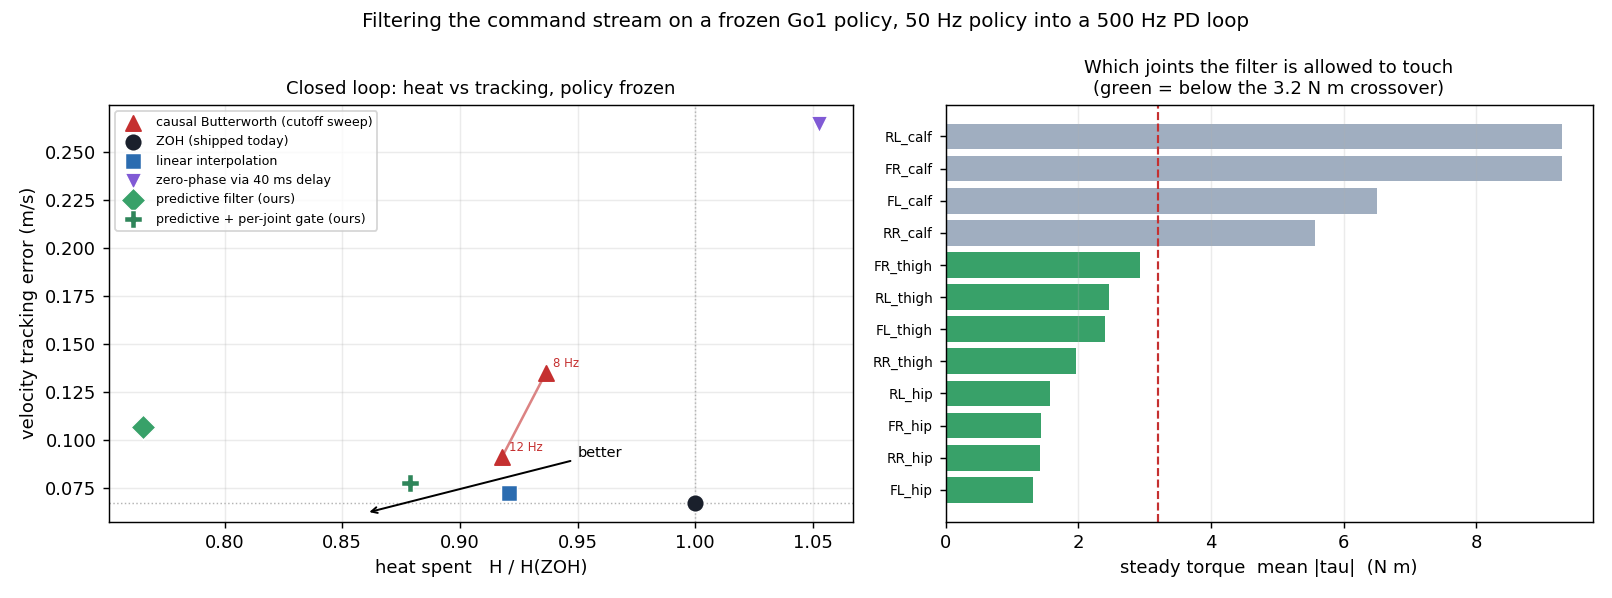
\includegraphics[width=0.82\textwidth]{figs/e4-closed-loop-no-torques-energy.png}
\caption{Closed loop, effort terms removed. The same matrix on the wasteful
policy. The predictive filter moves much further left; the delayed filter moves
off the chart to the right.}
\label{fig:closedloop2}
\end{figure*}
\fi

Removing effort terms inflates baseline dissipation by 47\% and increases the
reachable budget from 18.1\% to 43.3\%. The predictive filter recovers 47\% and
54\% of this reachable pool across the two policies, respectively. While raw
thermal savings differ by nearly $3\times$, 8.5\% against 23.5\%, the recovery
ratio remains invariant.

\subsection{Practical Guidelines}

Four rules follow. \emph{Profile before intervening}: one baseline rollout gives
the reachable budget and halving it estimates the closed-loop recovery, so a small
reachable share means the effort belongs in posture or reward rather than in a
filter. \emph{Do not buy zero phase with delay}: latency is taken out of the
policy's own phase margin, and the resulting falls appear only at the top of the
speed range, which is therefore where a candidate filter must be evaluated.
\emph{Gate by load}: restrict smoothing to joints below $\bar{\tau} \approx
\sqrt{\mathrm{Var}(\tau)}$, preserving tracking on stance joints while removing
jitter from unloaded ones. \emph{Prefer effort regularization to
\texttt{action\_rate}}: torque and energy penalties govern 89\% of the transient
against 8\%. Impact-mitigation rewards~\cite{impactmit} and compliant
feet~\cite{compliantfeet} reach the same budget from the reward and mechanical
sides respectively.

\section{Related Work}

\textbf{Thermal-aware locomotion.} Recent frameworks add motor temperature
observations and thermal reward bounds, train thermal residual policies, or use
contact-constrained inverse kinematics for multi-limbed humanoid thermal
balancing~\cite{thermalaware,residual,jorgensen}. All require complete retraining;
we instead characterize what a post-hoc intervention on a frozen checkpoint can
and cannot do.

\textbf{Command interfaces, smoothness, and control rate.} Interfaces bridging
high-level commands and motor drives include actuator reality shaping,
high-frequency torque interpolation, voltage-realizable acceleration bounds,
action-chunk post-optimization, B-spline policy representations, and forward delay
compensation~\cite{yamamori,kourdis,vra,lipo,bspline,weddington}. Manipulation
meets the same interface from the other side: action chunking runs a slow policy
above a fast controller~\cite{act} and receding-horizon diffusion execution makes
the chunk boundary the analogue of the ZOH step~\cite{diffusion}. Where the
actuator gap is treated as a modelling problem instead, the standard answers are
domain randomization, online system identification, and folding actuator limits
into training~\cite{domainrand,uposi,actconstrained}; all three require
retraining. Smoothness is
otherwise pursued during training, through CAPS, Lipschitz-constrained
architectures and spectral
normalization~\cite{caps,lipschitz,specnorm,benchmark}, through locally Lipschitz
continuity constraints, redesigned smoothing regularizers, stabilized
$Q$-gradient fields, and task-specified compliance
bounds~\cite{l2c2,regsmooth,qgrad,compliancebounds}, while the control-rate
literature reports robust locomotion at 8\,Hz, Q-learning degeneration as the time
step shrinks, and policies that choose their own action
durations~\cite{gangapurwala,tallec,tarc}, and the delayed-MDP literature maps
where such latency can and cannot be absorbed~\cite{delaysurvey}. None of this
work measures physical
copper loss or separates steady holding torque from command ripple, which is the
gap addressed here.

\section{Conclusion}

Actuator thermal overload in learned legged locomotion decomposes into
steady-state posture torque and dynamic command ripple. Because these components
add in quadrature, command filtering provides thermal relief only on lightly
loaded joints operating below the analytical crossover. In closed-loop execution,
filter phase lag directly degrades stability margins at operating speeds.
Consequently, causal predictive filtering with load-dependent gating provides a
reliable framework to recover actuator thermal margins on frozen checkpoints
without retraining.

This study is simulation only: squared torque proxies winding copper loss under
constant $K_t$, omitting iron losses, inverter switching and thermal diffusion,
so a lumped-parameter or learned thermal network would be required to turn the
proxy into a winding temperature~\cite{tnn};
single-joint sweeps omit contact dynamics; and every result is measured on flat
terrain on one quadruped. The 5\,Hz gait split is hand-chosen and has not been
swept, and the reward ablations are single-seed over 8\,s with no confidence
intervals. Extending the decomposition to a humanoid such as the Unitree G1, and
confirming the $3.2\Nm$ crossover on a dynamometer, are the essential next steps.

\balance
\begin{thebibliography}{99}
\footnotesize
\itemsep 0pt \parskip 0pt \parsep 0pt \labelsep 3pt

\bibitem{lee}
J. Lee, J. Hwangbo, L. Wellhausen, V. Koltun, and M. Hutter, ``Learning
quadrupedal locomotion over challenging terrain,'' \emph{Science Robotics},
vol. 5, no. 47, eabc5986, 2020.

\bibitem{miki}
T. Miki, J. Lee, J. Hwangbo, L. Wellhausen, V. Koltun, and M. Hutter, ``Learning
robust perceptive locomotion for quadrupedal robots in the wild,'' \emph{Science
Robotics}, vol. 7, no. 62, eabk2822, 2022.

\bibitem{g1issue}
NVIDIA Research, ``Ankle roll motors overheating on G1,''
GR00T-WholeBodyControl, GitHub issue \#174, 2026.

\bibitem{go2w}
T. Matsuzawa, K. Irie, T. Yoshida, T. Suzuki, Y. Hara, and M. Tomono,
``Long-distance real-world navigation of the legged-wheeled robot Go2-W using
deep reinforcement learning,'' arXiv:2606.21387, 2026.

\bibitem{resourceconstrained}
\pending, ``Robust reinforcement learning-based locomotion for
resource-constrained quadrupeds with exteroceptive sensing,'' arXiv:2505.12537,
2025.

\bibitem{wensing}
P. M. Wensing, A. Wang, S. Seok, D. Otten, J. Lang, and S. Kim, ``Proprioceptive
actuator design in the MIT Cheetah: Impact mitigation and high-bandwidth physical
interaction for dynamic legged robots,'' \emph{IEEE Trans. Robot.}, vol. 33,
no. 3, pp. 509--522, 2017.

\bibitem{minicheetah}
B. Katz, J. Di Carlo, and S. Kim, ``Mini Cheetah: A platform for pushing the
limits of dynamic quadruped control,'' in \emph{Proc. ICRA}, 2019.

\bibitem{anymal}
M. Hutter et al., ``ANYmal --- a highly mobile and dynamic quadrupedal robot,''
in \emph{Proc. IROS}, 2016.

\bibitem{hwangbo}
J. Hwangbo et al., ``Learning agile and dynamic motor skills for legged robots,''
\emph{Science Robotics}, vol. 4, no. 26, eaau5872, 2019.

\bibitem{unitreesdk}
Unitree Robotics, ``unitree\_legged\_sdk,''
\texttt{example\_py/\allowbreak example\_position.py}, GitHub, 2024.

\bibitem{lite3blog}
DEEP Robotics, ``Physical AI 101: reinforcement learning with the Lite3,''
company blog, 2025.

\bibitem{gom8010}
Unitree Robotics, ``GO-M8010-6 motor data user manual,'' V1.0, 2023.

\bibitem{j60}
DEEP Robotics, ``J60 joint,'' product page, 2024.

\bibitem{mjlab}
K. Zakka, Q. Liao, B. Yi, L. Le Lay, K. Sreenath, and P. Abbeel, ``mjlab: A
lightweight framework for GPU-accelerated robot learning,'' arXiv:2601.22074,
2026.

\bibitem{orbit}
M. Mittal et al., ``Orbit: A unified simulation framework for interactive robot
learning environments,'' \emph{IEEE Robot. Autom. Lett.}, 2023.

\bibitem{maxon}
maxon motor ag, ``EC max 30 \O30\,mm, brushless, 60\,W,'' datasheet, 2024.

\bibitem{wallscheid}
O. Wallscheid, ``Thermal monitoring of electric motors: State-of-the-art review
and future challenges,'' \emph{IEEE Open J. Ind. Appl.}, 2021.

\bibitem{kirchgassner}
W. Kirchg\"{a}ssner, O. Wallscheid, and J. B\"{o}cker, ``Estimating electric motor
tem\-per\-a\-tures with deep resid\-ual ma\-chine learn\-ing,'' \emph{IEEE Trans. Power
Electron.}, vol. 36, no. 7, pp. 7480--7488, 2021.

\bibitem{thermalpred}
\pending, ``Deep learning for model-free prediction of thermal states of robot
joint motors,'' arXiv:2509.12739, 2025.

\bibitem{urs}
K. Urs, C. E. Adu, E. J. Rouse, and T. Y. Moore, ``Design and characterization of
3D printed, open-source actuators for legged locomotion,'' in \emph{Proc. IROS},
2022.

\bibitem{energymotor}
\pending, ``Energy efficient control of electric motors,'' arXiv:2109.11113,
2021.

\bibitem{cliff}
N. Cliff, ``Dominance statistics: Ordinal analyses to answer ordinal questions,''
\emph{Psychol. Bull.}, vol. 114, no. 3, pp. 494--509, 1993.

\bibitem{rudin}
N. Rudin, D. Hoeller, P. Reist, and M. Hutter, ``Learning to walk in minutes
using massively parallel deep reinforcement learning,'' in \emph{Proc. CoRL},
2022.

\bibitem{isaacgym}
V. Makoviychuk et al., ``Isaac Gym: High performance GPU-based physics simulation
for robot learning,'' arXiv:2108.10470, 2021.

\bibitem{wtw}
G. B. Margolis and P. Agrawal, ``Walk these ways: Tuning robot control for
generalization with multiplicity of behavior,'' in \emph{Proc. CoRL}, 2023,
pp. 22--31.

\bibitem{playground}
K. Zakka et al., ``MuJoCo Playground,'' arXiv:2502.08844, 2025.

\bibitem{makhoul}
J. Makhoul, ``Linear prediction: A tutorial review,'' \emph{Proc. IEEE}, vol. 63,
no. 4, pp. 561--580, 1975.

\bibitem{harris}
F. J. Harris, ``On the use of windows for harmonic analysis with the discrete
Fourier transform,'' \emph{Proc. IEEE}, vol. 66, no. 1, pp. 51--83, 1978.

\bibitem{motorselect}
\pending, ``Alternative metrics to select motors for quasi-direct drive
actuators,'' arXiv:2202.12365, 2022.

\bibitem{energyreg}
\pending, ``Adaptive energy regularization for autonomous gait transition and
energy-efficient quadruped locomotion,'' arXiv:2403.20001, 2024.

\bibitem{gustafsson}
F. Gustafsson, ``Determining the initial states in forward-backward filtering,''
\emph{IEEE Trans. Signal Process.}, vol. 44, no. 4, pp. 988--992, 1996.

\bibitem{concurrent}
\pending, ``Concurrent training of a control policy and a state estimator for
dynamic and robust legged locomotion,'' arXiv:2202.05481, 2022.

\bibitem{delayaware}
B. Chen, M. Xu, L. Li, and D. Zhao, ``Delay-aware model-based reinforcement
learning for continuous control,'' \emph{Neurocomputing}, vol. 450,
pp. 119--128, 2021.

\bibitem{rtc}
K. Black et al., ``Real-time execution of action chunking flow policies,'' in
\emph{Proc. NeurIPS}, 2025.

\bibitem{impactmit}
\pending, ``Guiding energy-efficient locomotion through impact mitigation
rewards,'' arXiv:2510.09543, 2025.

\bibitem{compliantfeet}
\pending, ``Energy-efficient quadruped locomotion with compliant feet,''
arXiv:2605.14411, 2026.

\bibitem{thermalaware}
\pending, ``Learning thermal-aware locomotion policies for an
electrically-actuated quadruped robot,'' arXiv:2603.01631, 2026.

\bibitem{residual}
Y. Wan, W. Lin, L. Qian, Y. Zou, W. Wu, S. Liao, C. Zhao, and X. Luo, ``Learning
to balance motor thermal safety and quadrupedal locomotion performance with
residual policy,'' arXiv:2605.27046, 2026.

\bibitem{jorgensen}
S. J. Jorgensen, J. Holley, F. Mathis, J. S. Mehling, and L. Sentis, ``Thermal
re\-cov\-ery of multi-limbed ro\-bots with elec\-tric ac\-tu\-a\-tors,'' \emph{IEEE Robot.
Autom. Lett.}, vol. 4, no. 2, pp. 1077--1084, 2019.

\bibitem{yamamori}
S. Yamamori et al., ``Actuator reality shaping for zero-shot sim-to-real robot
learning,'' arXiv:2607.02205, 2026.

\bibitem{kourdis}
R. Kourdis, M. St\k{e}pie\'{n}, J. Manhes, N. Mansard, S. Tonneau, P. Sou\`{e}res,
and T. Flayols, ``Very high frequency interpolation for direct torque control,''
arXiv:2509.24175, 2025.

\bibitem{vra}
L. Zhang, J. Wang, T. Zhang, Z. Song, X. Zeng, W. Xia, Z. Li, and Y. Liu, ``VRA:
Grounding discrete-time joint acceleration in voltage-constrained actuation,'' in
\emph{Proc. RSS}, 2026.

\bibitem{lipo}
D. Son and S. Park, ``LiPo: A lightweight post-optimization framework for
smoothing action chunks generated by learned policies,'' arXiv:2506.05165, 2025.

\bibitem{bspline}
X. Han, H. Xiong, H. Chen, C. Liu, A. Torralba, Y. Zhu, and Y. Du, ``B-spline
policy: Accelerating manipulation policies via B-spline action representations,''
arXiv:2607.09648, 2026.

\bibitem{weddington}
J. C. Weddington, B. P. \"{O}lveczky, and S. A. Baccus, ``Reinforcement learning
on cost-constrained quadrupedal hardware,'' arXiv:2607.26434, 2026.

\bibitem{act}
T. Z. Zhao, V. Kumar, S. Levine, and C. Finn, ``Learning fine-grained bimanual
manipulation with low-cost hardware,'' arXiv:2304.13705, 2023.

\bibitem{diffusion}
C. Chi, Z. Xu, S. Feng, E. Cousineau, Y. Du, B. Burchfiel, R. Tedrake, and
S. Song, ``Diffusion policy: Visuomotor policy learning via action diffusion,''
\emph{Int. J. Robot. Res.}, 2025.

\bibitem{domainrand}
J. Tobin, R. Fong, A. Ray, J. Schneider, W. Zaremba, and P. Abbeel, ``Domain
randomization for transferring deep neural networks from simulation to the real
world,'' arXiv:1703.06907, 2017.

\bibitem{uposi}
W. Yu, J. Tan, C. K. Liu, and G. Turk, ``Preparing for the unknown: Learning a
universal policy with online system identification,'' in \emph{Proc. RSS}, 2017.

\bibitem{actconstrained}
\pending, ``Actuator-constrained reinforcement learning for high-speed
quadrupedal locomotion,'' arXiv:2312.17507, 2023.

\bibitem{caps}
S. Mysore, B. Mabsout, R. Mancuso, and K. Saenko, ``Regularizing action policies
for smooth control with reinforcement learning,'' in \emph{Proc. ICRA}, 2021.

\bibitem{lipschitz}
Z. Chen et al., ``Learning smooth humanoid locomotion through
Lipschitz-constrained policies,'' in \emph{Proc. IROS}, 2025.

\bibitem{specnorm}
J. Shin, W. Cha, D. Kim, J. Cha, and J. Park, ``Spectral normalization for
Lipschitz-constrained policies on learning humanoid locomotion,''
arXiv:2504.08246, 2025.

\bibitem{benchmark}
G. Christmann, Y. Luo, H. Mandala, and W. Chen, ``Benchmarking smoothness and
reducing high-frequency oscillations in continuous control policies,'' in
\emph{Proc. IROS}, 2024.

\bibitem{l2c2}
\pending, ``L2C2: Locally Lipschitz continuous constraint towards stable and
smooth reinforcement learning,'' arXiv:2202.07152, 2022.

\bibitem{regsmooth}
\pending, ``Redesigning regularization for effective policy smoothing,''
arXiv:2606.13169, 2026.

\bibitem{qgrad}
\pending, ``Stabilizing the Q-gradient field for policy smoothness in
actor-critic methods,'' arXiv:2601.22970, 2026.

\bibitem{compliancebounds}
\pending, ``Task-specified compliance bounds for humanoids via
Lipschitz-constrained policies,'' arXiv:2603.16180, 2026.

\bibitem{gangapurwala}
S. Gangapurwala, L. Campanaro, and I. Havoutis, ``Learning low-frequency motion
control for robust and dynamic robot locomotion,'' in \emph{Proc. ICRA}, 2023.

\bibitem{tallec}
C. Tallec, L. Blier, and Y. Ollivier, ``Making deep Q-learning methods robust to
time discretization,'' in \emph{Proc. ICML}, 2019.

\bibitem{tarc}
A. Sukhija, L. Treven, J. Cheng, F. D\"{o}rfler, S. Coros, and A. Krause, ``TARC:
Time-adaptive robotic control,'' arXiv:2510.23176, 2025.

\bibitem{delaysurvey}
\pending, ``Delays in reinforcement learning,'' arXiv:2309.11096, 2023.

\bibitem{tnn}
W. Kirchg\"{a}ssner et al., ``Thermal neural networks: Lumped-parameter thermal
modeling with state-space machine learning,'' arXiv:2103.16323, 2021.

\end{thebibliography}

\end{document}
